\begin{tcolorbox}[posterbox]
\SectionTitle{EEG Acquisition and Processing}
\SmallText
\textbf{Recording \& Preprocessing}
\begin{itemize}
  \item 128-channel EGI Geodesic Sensor Net (250 Hz sampling rate).
  \item Bandpass filtered 0.1--100 Hz (online); low-pass 40 Hz (offline); re-referenced to average.
  \item Epochs segmented $-100$ to $600$ ms relative to target onset.
\end{itemize}

\textbf{Analysis Windows \& Montages}
\begin{itemize}
  \item \textbf{P1 (80--120 ms) \& N1 (125--200 ms):} Bilateral POT junction.
    Left: 66, 65, 59, 60, 67, 71, 70;\quad Right: 84, 76, 77, 85, 91, 90, 83.
  \item \textbf{P3b (435--535 ms):} Midline Parietal (Pz). Electrodes: 62, 78, 77, 72, 67, 61, 54, 55, 79.
  \item \textbf{MMN (100--120 ms):} Midline Frontal (Fz); indexes automatic numerical change detection.
\end{itemize}

\begin{center}
  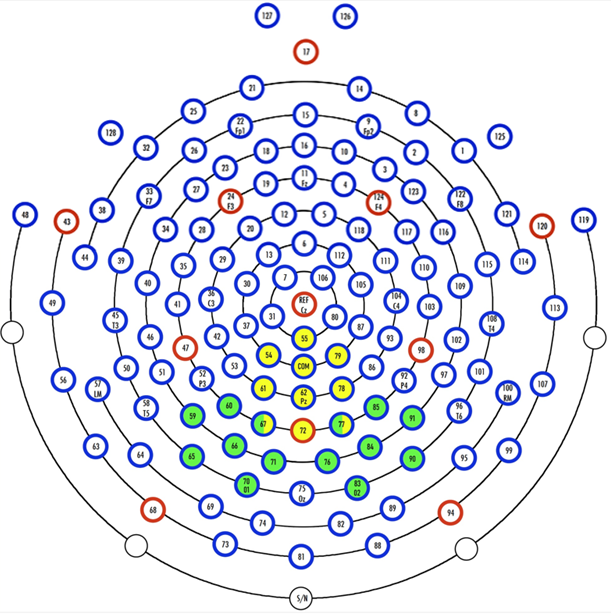
\includegraphics[width=0.56\linewidth, height=11in, keepaspectratio]{media/electrodes.png}
\end{center}
\SmallText
\textbf{Fig. 2.} Electrode map used for POT and midline analyses.
\end{tcolorbox}

\vspace{0.06in}

\begin{tcolorbox}[posterbox]
\SectionTitle{Statistical Analyses}
\SmallText
\textbf{Behavioral Data}
\begin{itemize}
  \item Log-transformed RT modeled with \textbf{Generalized Estimating Equations (GEE)} using an exchangeable working covariance, accounting for within-subject dependence.
  \item Accuracy modeled via \textbf{logistic GEE}; odds ratios reported with 95\% confidence intervals.
  \item Subject-level effects confirmed with paired $t$-tests on individual slopes and mean differences.
\end{itemize}

\textbf{ERP Data}
\begin{itemize}
  \item Mean amplitude extracted within each component window (P1, N1, MMN, P3b) per participant per condition.
  \item Condition contrasts tested with \textbf{linear mixed models}; Bonferroni correction applied for multiple comparisons.
  \item Epoch acceptance threshold: $\pm 100\,\mu\mathrm{V}$; artifact epochs excluded prior to averaging.
\end{itemize}

\begin{center}
{\renewcommand{\arraystretch}{1.35}
\begin{tabular}{@{}llll@{}}
\toprule
\textbf{Component} & \textbf{Window} & \textbf{Region} & \textbf{Reflects} \\
\midrule
P1   & 80--120 ms   & Bilateral POT & Early visual encoding \\
N1   & 125--200 ms  & Bilateral POT & Sensory discrimination \\
MMN  & 100--120 ms  & Frontal (Fz)  & Auto.\ change detection \\
P3b  & 435--535 ms  & Parietal (Pz) & WM updating \\
\bottomrule
\end{tabular}}
\end{center}
\end{tcolorbox}
